
%(BEGIN_QUESTION)
% Copyright 2006, Tony R. Kuphaldt, released under the Creative Commons Attribution License (v 1.0)
% This means you may do almost anything with this work of mine, so long as you give me proper credit

Explain the meaning of Faraday's Law of electromagnetic induction, shown in this familiar equation:

$$e = N {d \Phi \over dt}$$

Then, explain the meaning of this {\it other} version of Faraday's Law of electromagnetic induction, the voltage described by it often being referred to as a {\it motional EMF}:

$$e = Blv$$

\underbar{file i00521}
%(END_QUESTION)





%(BEGIN_ANSWER)

$$e = N {d \Phi \over dt}$$

\noindent
Where,

$e$ = Instantaneous voltage induced in a wire coil

$N$ = Number of turns of wire in the coil

$d \Phi \over dt$ = Instantaneous rate of change of magnetic flux over time

\vskip 20pt

$$e = Blv$$

\noindent
Where,

$e$ = Instantaneous voltage induced along a straight wire

$B$ = Magnetic flux density

$l$ = Length of wire

$v$ = Velocity of wire

%(END_ANSWER)





%(BEGIN_NOTES)

Recall that $B$ is flux density, defined as the concentration of magnetic flux per unit area ($B = {\Phi \over A}$).  We can also say that $\Phi = B A$, or more properly (using vector variables\footnote{$^{1}$}{In this analysis, I will blatantly ignore signs for reasons of simplicity.}) that $\Phi = \int \vec B \cdot d \vec A$.  By substitution, we may re-write the first version of Faraday's Law as such:

$$e = N {d \over dt} \int \vec B \cdot d \vec A$$

A straight wire of length $l$ moving perpendicularly to its length covers an area $A$ equal to $lx$:

$$\includegraphics[width=15.5cm]{i00521x01.eps}$$

Expressing $A$, $l$, and $x$ as vectors, we may say that $\vec A = \vec l \times \vec x$.  If $l$ is constant (which it should be!), the equation $\vec A = \vec l \times \vec x$ may be differentiated like this:

$$d \vec A = \vec l \times d \vec x$$

Next, we substitute $\vec l \times d \vec x$ for $d \vec A$ in the integrand of Faraday's equation:

$$e = N {d \over dt} \int \vec B \cdot (\vec l \times d \vec x)$$

Of course, we know that velocity $v$ is the time-derivative of distance $x$:

$$v = {dx \over dt} \hbox{\hskip 30pt . . . or . . . \hskip 30pt} dx = v \> dt$$

Now, we substitute $\vec v \> dt$ for $d \vec x$ in the integrand of Faraday's equation:

$$e = N {d \over dt} \int \vec B \cdot (\vec l \times \vec v) \> dt$$

The differentiation and integration simply cancel one another, both being made with respect to time $t$:

$$e = N \vec B \cdot (\vec l \times \vec v)$$

If there is only one wire involved, $N = 1$ and we may re-write like this:

$$e = \vec B \cdot (\vec l \times \vec v)$$

If we know that the velocity vector ($\vec v$) is perpendicular to the length vector ($\vec l$), then the cross-product ($\vec A$) must be perpendicular to both.  If both $\vec v$ and $\vec l$ are perpendicular to the magnetic field vector ($\vec B$), the area vector ($\vec A$) must be parallel to the field vector and the dot product becomes equal to the scalar product:

$$e = Blv$$

%INDEX% Physics, electricity: Faraday's law of electromagnetic induction

%(END_NOTES)


